%!TEX root = tesis.tex
\chapter{Aprendizaje en un \ssolver paralelo y distribuido}
\label{aprendizaje-pardist}

En el Cap.~\ref{ssolver-pardist} vimos que el enfoque de distribución aplicado
consigue disminuir el tiempo necesario para resolver una serie de problemas de
tamaño considerable. Al mismo tiempo observamos que existen casos en los que
la eficiencia --entendida como cuánto ganamos por cada unidad de \hard
agregada al cómputo de un problema-- resulta pobre. Planteamos como hipótesis
que esta situación se debe, en gran medida, a una importante cantidad de
retrabajo que se produce como consecuencia del particionado de un problema en
diversos subproblemas. 

La existencia de retrabajo se evidencia en que si bien al partir un problema
en subproblemas, el subproblema más grande suele ser más chico que el padre,
la suma del tiempo requerido para resolver todos los subproblemas hijos es
considerablemente mayor que el tiempo requerido para resolver el problema
padre. Debido al esquema de particionado recursivo, este incremento en el
tiempo total de cómputo requerido para resolver un problema se vuelve
sustancial.

En el presente capítulo desarrollaremos un mecanismo de reutilización del
conocimiento adquirido durante la ejecución de cada subproblema. Este
mecanismo persigue dos objetivos principales: verificar la hipótesis planteada
y, de ser posible,  disminuir los tiempos requeridos para resolver un problema
aumentando la eficiencia de la herramienta.

\section{Justificación del enfoque}

El enfoque de particionamiento recursivo, basado en \emph{guiding paths}, que
hemos adoptado para la construcción de la herramienta también influye en la
elección de un mecanismo adecuado para compartir información de cláusulas
aprendidas. 

\newcommand{\roottask}{\ensuremath{<\varphi_R, \emptyset>}\xspace}
\newcommand{\task}{\ensuremath{<\varphi, \emptyset>}\xspace}
\newcommand{\nonemptytask}{\ensuremath{<\varphi, C>}\xspace}

Consideremos ahora que un problema no es ya únicamente una fórmula $\varphi$
sino una tupla $<\varphi, C>$ donde $C$ es un conjunto de cláusulas tales que
$(\forall v) (v \models \varphi \Longleftrightarrow v \models \varphi
\bigwedge C)$ llamado conjunto de cláusulas aprendidas. En este contexto el
problema original es la tupla \roottask donde $\varphi_R$ denota la fórmula
original que se desea verificar. En este modelo, al partir un problema \task
levantando (por ejemplo) la variable $u$ obtenemos dos nuevos subproblemas
$<\varphi_u, \emptyset>$ y $<\varphi_{-u}, \emptyset>$. 

Notemos entonces que dado un problema \nonemptytask podemos generar los
subproblemas que resultan de levantar la variable $u$ como sigue:
$t_u=<\varphi_u, C_u>$ y $t_{-u}=<\varphi_{-u}, C_{-u}>$ (donde $C_u$ es el
conjunto de cláusulas que resulta de reemplazar las apariciones de la variable
$u$ por el valor $1$ en el conjunto $C$ y $C_{-u}$ es el resultado de
reemplazar las apariciones de la variable $u$ por el valor $0$) sin alterar la
corrección de la herramienta. Esto se debe a que si $v \models \varphi_u$
entonces $v\cup\{u\leftarrow1\} \models \varphi$ y por lo tanto
$v\cup\{u\leftarrow1\} \models \varphi \bigwedge C$ de lo que se deduce que $v
\models \varphi_u \bigwedge C_u$. Lo mismo vale para el caso $\varphi_{-u}$.

Más aún, lo antedicho vale también para cualquier subconjunto de $C$. Esto
induce una manera \emph{natural} de reutilización de las cláusulas aprendidas
que llamaremos \emph{herencia}. Este mecanismo consiste en que al generar
nuevos subproblemas a partir de un problema padre \nonemptytask, los
subproblemas hijos son generados con un subconjunto de $C$ como conjunto de
cláusulas aprendidas. Llamaremos \emph{criterio} a cada forma distinta de
obtener un subconjunto a partir de un conjunto de cláusulas $C$.


\subsubsection{Consideraciones de escalabilidad}

Además de la naturalidad inducidad por el esquema de particionado, nos
interesa también evitar cualquier enfoque que introduzca nuevos cuellos de
botella en la arquitectura. Por ejemplo, no sería aceptable la incorporación
de una gran base de datos centralizada en la que todos los \ws almacenen las
cláusulas que van aprendiendo y que todos los \ws deban consultar.

Tampoco sería aceptable un grafo completo de comunicación permanente para
lograr ese mismo fin, es decir, hacer que cada \w le comunique (o consulte) a
todos los demás las cláusulas que va(n) aprendiendo.


\subsubsection{Independencia del \ssolver particular utilizado}

Por otro lado, como ya hemos señalado en el Cap.~\ref{ssolver-pardist}, nos
interesa que el \ssolver secuencial que utiliza cada uno de los \ws sea fácil
de actualizar y/o de reemplazar por otro componente \ots similar. Si bien
suelen ser necesarios algunos cambios para lograr que un \ssolver permita la
inyección \emph{inicial} de cláusulas aprendidas (en lugar de comenzar sin
ninguna), por lo general tales cambios se reducen a cuestiones de interfaz y
no revisten mayor dificultad.

Es más ambicioso, en cambio, pretender poder inyectar nuevas cláusulas
aprendidas en cualquier momento \emph{durante} el proceso de búsqueda. Para
ello habría que introducir modificaciones mucho más fuertemente acopladas a la
versión particular de \ssolver en uso, sus algoritmos, estructuras de datos e
invariantes particulares.

\

Es por estos factores que optamos por implementar un esquema de reutilización
de cláusulas aprendidas basado en herencia. En esencia el esquema funciona de
acuerdo a lo detallado al comienzo de esta sección. En particular, a la hora
de partir un problema en nuevos subproblemas un \emph{criterio} es aplicado al
conjunto de cláusulas aprendidas que el problema padre poseía al momento de
ser abortado. De esta manera se generan los subconjuntos de cláusulas
aprendidas que los subproblemas hijos deberán incorporar antes de comenzar el
análisis. Cabe destacar que si bien la herramienta permite seleccionar un
nuevo criterio de aprendizaje cada vez que un problema es partido, en la
evaluación realizada no se utilizó esta característica sino que se mantuvo un
mismo criterio para toda la corrida.


\subsubsection{Sobre los criterios}

En principio podríamos preguntarnos de dónde surge la necesidad de tener
criterios para la herencia de cláusulas aprendidas. O lo que es lo mismo, por
qué no heredar todas las cláusulas aprendidas del padre. Existen varias
razones que motivan la necesidad de introducir criterios de selección de
cláusulas.

En primer lugar la incorporación de cláusulas aprendidas a un problema
incrementa la cantidad de cláusulas sobre las que es necesario propagar las
decisiones. Esto provoca una ralentización del proceso de propagación que
puede resultar en una disminución del rendimiento del \ssolver secuencial. La
información experimental presentada en diversos artículos muestra que,
incrementar en demasía la base de datos de cláusulas aprendidas en un \ssolver
secuencial, se torna contraproducente. Es por esto que los \ssolvers
secuenciales cuentan con políticas de recorte de dicha base de datos y que,
por lo general, estas políticas son bastante agresivas.

Otro factor que aboga en contra de mantener la totalidad de las cláusulas
aprendidas por el padre es el hecho de que los subproblemas generados suelen
ser más chicos que el padre. Incluso es bastante común que una buena
proporción de los subproblemas generados al partir un problema padre sean
considerablemente más chicos. En todos estos casos la incorporación de una
conjunto de cláusulas aprendidas extremadamente grande, resultará
inmediatamente contraproducente debido a lo expuesto en el párrafo anterior.

El último motivo para la introducción de criterios de selección es que el
conjunto de cláusulas aprendidas de un problema es potencialmente muy grande.
Por otro lado, los subproblemas generados no son resueltos inmediatamente sino
que pasan a formar parte de la cola de tareas pendientes. Es decir que,
heredar la totalidad de las cláusulas aprendidas del problema padre en cada
uno de los subproblemas hijos, nos obligaría a pagar un alto costo debido a la
escritura y posterior lectura --hacia y desde memoria secundaria-- de cada
unos de estos conjuntos (potencialmente muy grandes) más el costo de la
posible transmición por medio de la red. Esto atentaría directamente contra el
desempeño de nuestra herramienta, incrementando en demasía los costos
\emph{fijos} asociados al enfoque.

% Que cada hijo herede TODAS las cláusulas aprendidas por su padre probablemente sea demasiado / contraproducente:
% \begin{itemize}
% \item Por algo los solvers secuenciales van purgando: es sabido que zarparse no es bueno.
% \item OK, el padre sí llegó a todo eso, pero por algo los solvers secuenciales van subiendo de a poco el máximo de aprendidas: es sabido que zarparse desde el primer momento no es buena idea. Y estamos suponiendo que los subproblemas serán más chicos/fáciles que su problema padre.
% \item Y además, la herencia no es inmediata sino mediata. Jugarse a heredar todo implica jugarse a pagar el precio de bajar todo eso a disco, guardar todo eso en storage/pending, leer todo eso de disco, etc. Bocha overhead.
% \end{itemize}

% Por lo tanto vamos a necesitar criterios de selección, subconjunto, etc.


\section{Prueba de concepto}

Con el objetivo de evaluar la pertinencia y viabilidad del enfoque propuesto
para el aprendizaje, llevamos a cabo una prueba de concepto. 


Esta prueba de concepto consistió en la ejecución de distintos problemas
realizando una única partición y aplicando distintos criterios de selección de
cláusulas aprendidas y comparando los tiempos obtenidos. Para ello cada
problema fue ejecutado durante 60 segundos y luego partido levantando 5
variables para obtener 32 subproblemas. Cada uno de los subproblemas fue
ejecutado hasta su finalización. Para evitar la invalidez de los resultados
cada criterio fue testeado utilizando 10 órdenes pseudoaletorios distintos que
determinaron las variables levantadas en cada caso. Luego, se compararon tanto
los tiempos totales de cómputo invertidos en resolver el problema, como el
tiempo del camino crítico (determinado por el subproblema que más tiempo tomó).


\subsubsection{Resultados obtenidos}

Acá van los resultados de las perchitas.

\subsubsection{Discusión y conclusiones}

Acá discutimos los resultados y concluimos que vale la pena probar implementar
la herencia de cláusulas aprendidas en modo paralelo y distribuido, y
evaluarla en un cluster posta.


\section{Resultados experimentales}

En esta sección vamos a presentar los resultados posta de los experimentos
ejecutados en distribuido.

\subsection{Criterios de selección de cláusulas}

Descripción de los distintos criterios \ldots

\subsection{Resultados obtenidos}

\subsubsection{Garping del mejor criterio para cada problema}

\subsubsection{Promedios por cada criterio}

\subsubsection{Heatmaps para scopes crecientes}


\subsection{Discusión y conclusiones}


\newpage
% \begin{figure}
% 	\centering
% 	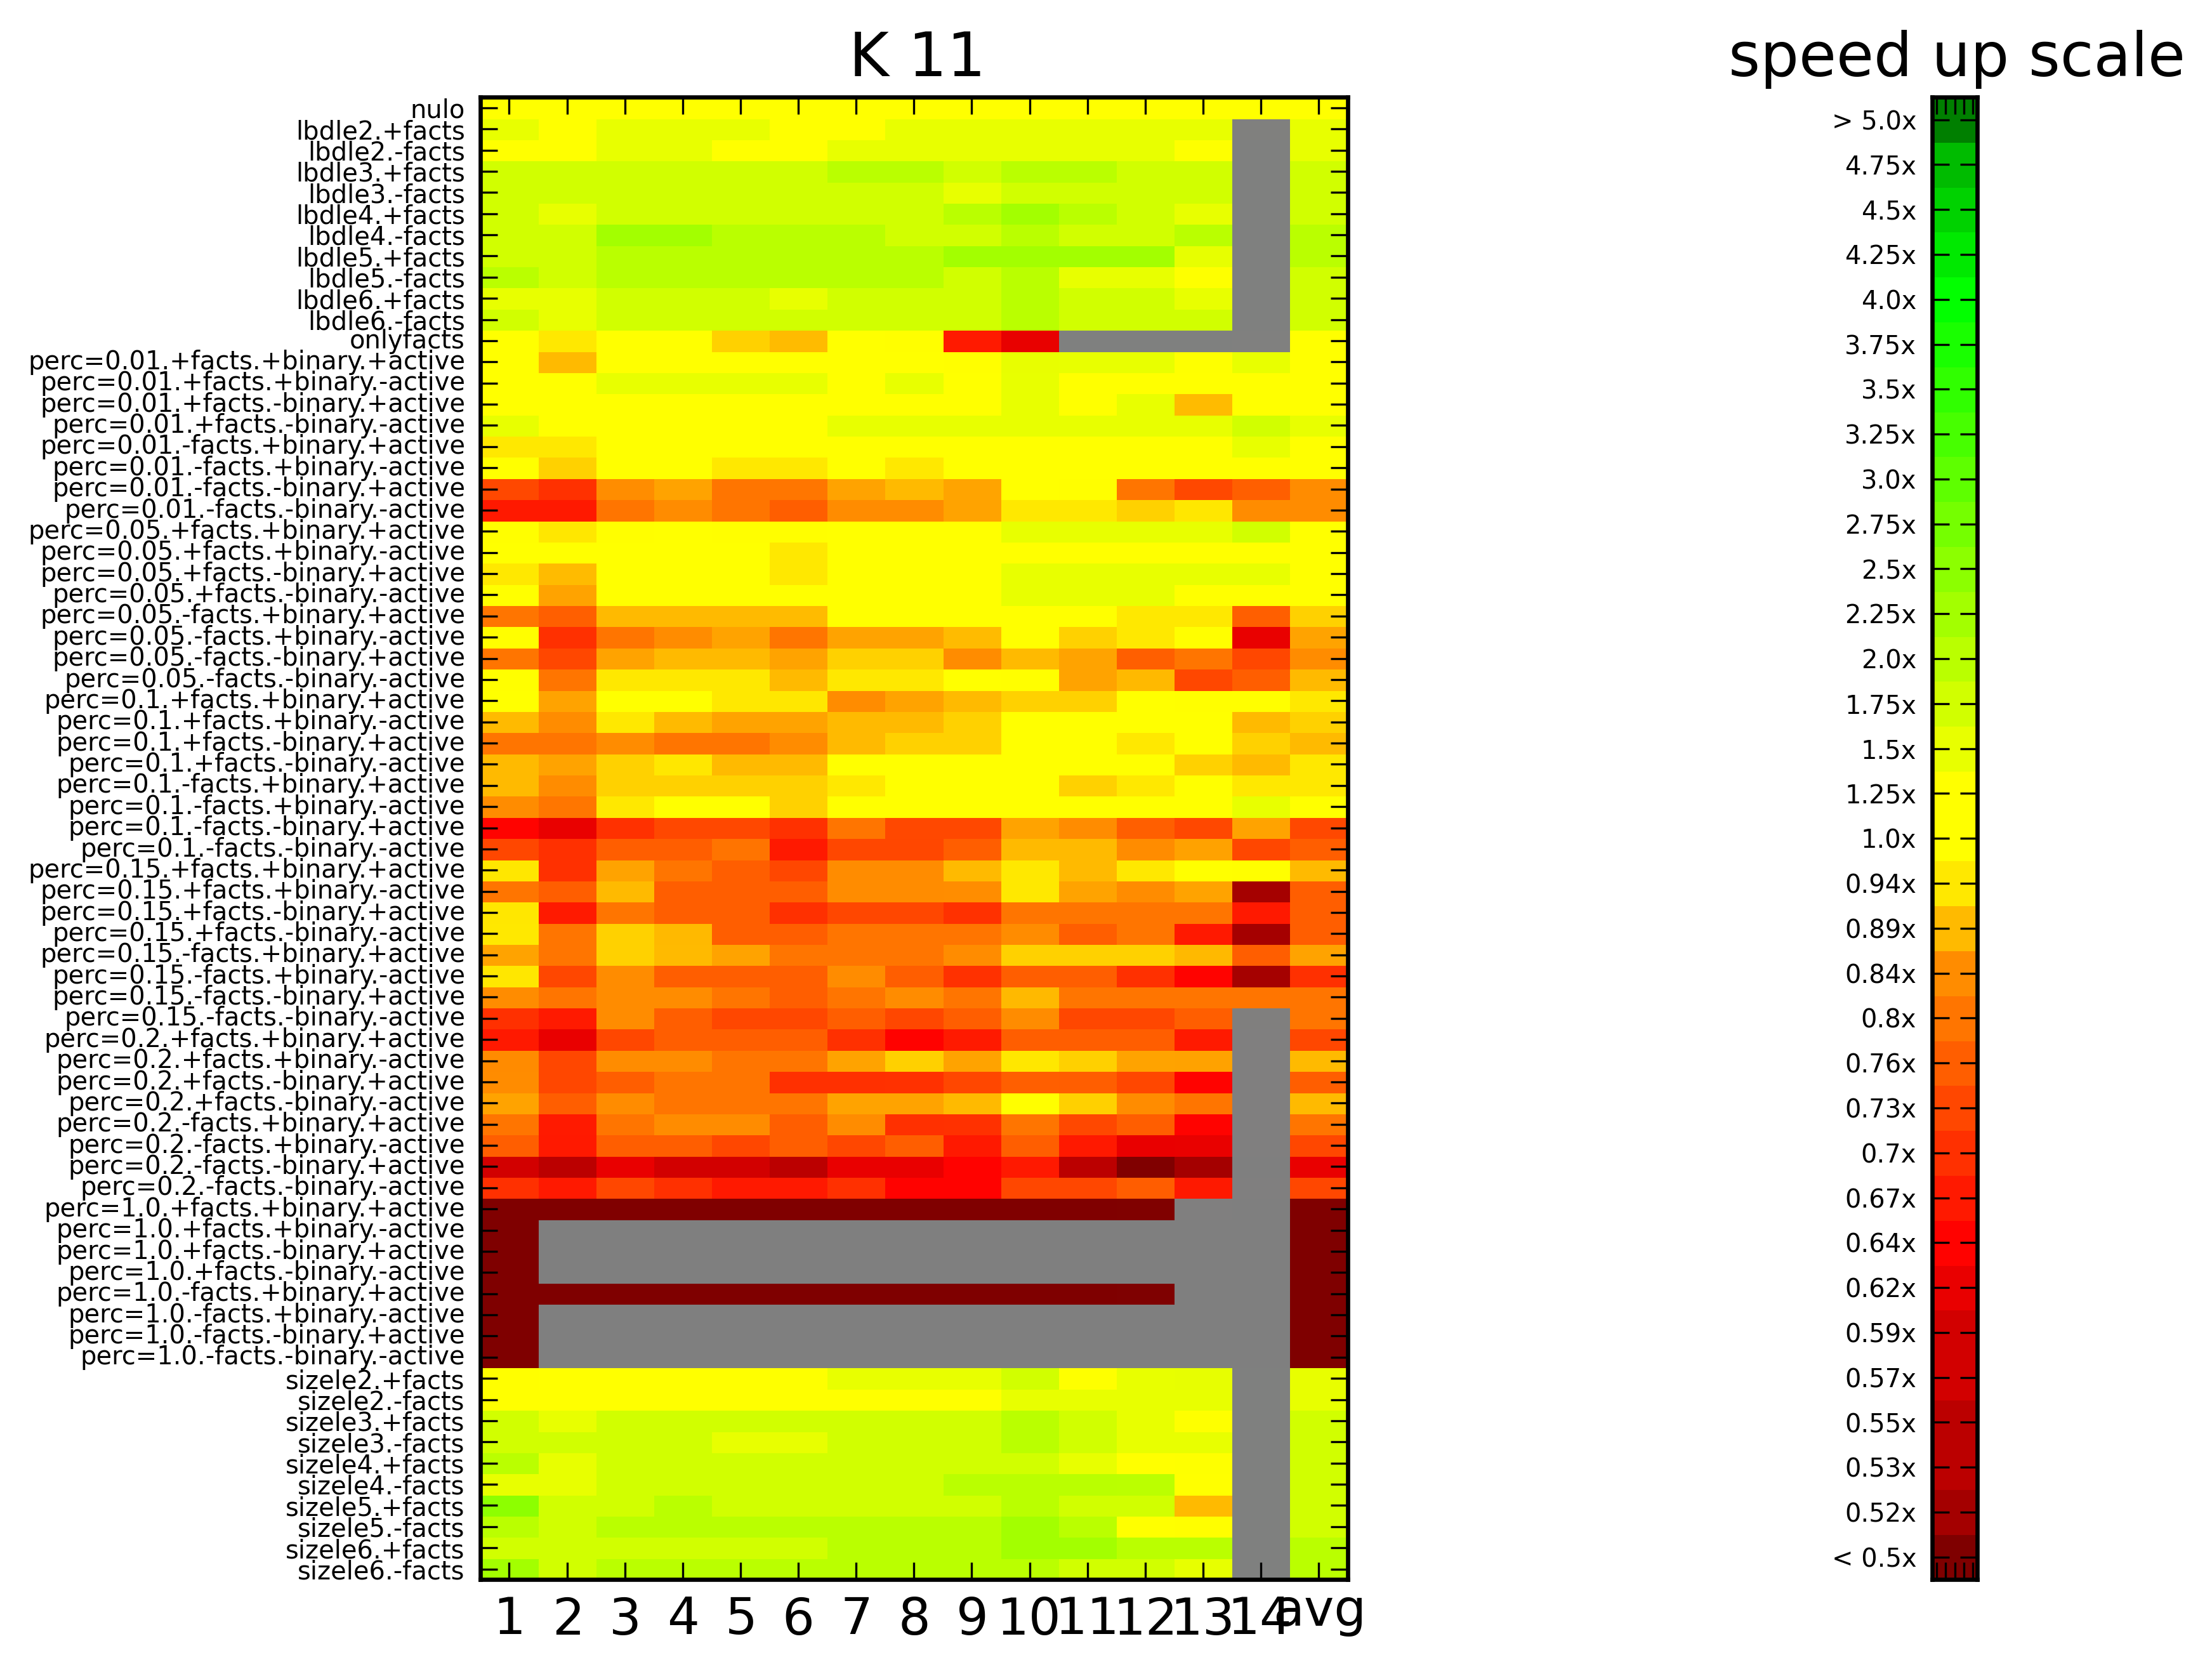
\includegraphics[scale=0.5]{resultados/k11_heat}
% 	%\caption{\emph{Workers}}
% \end{figure}
% \begin{figure}
% 	\centering
% 	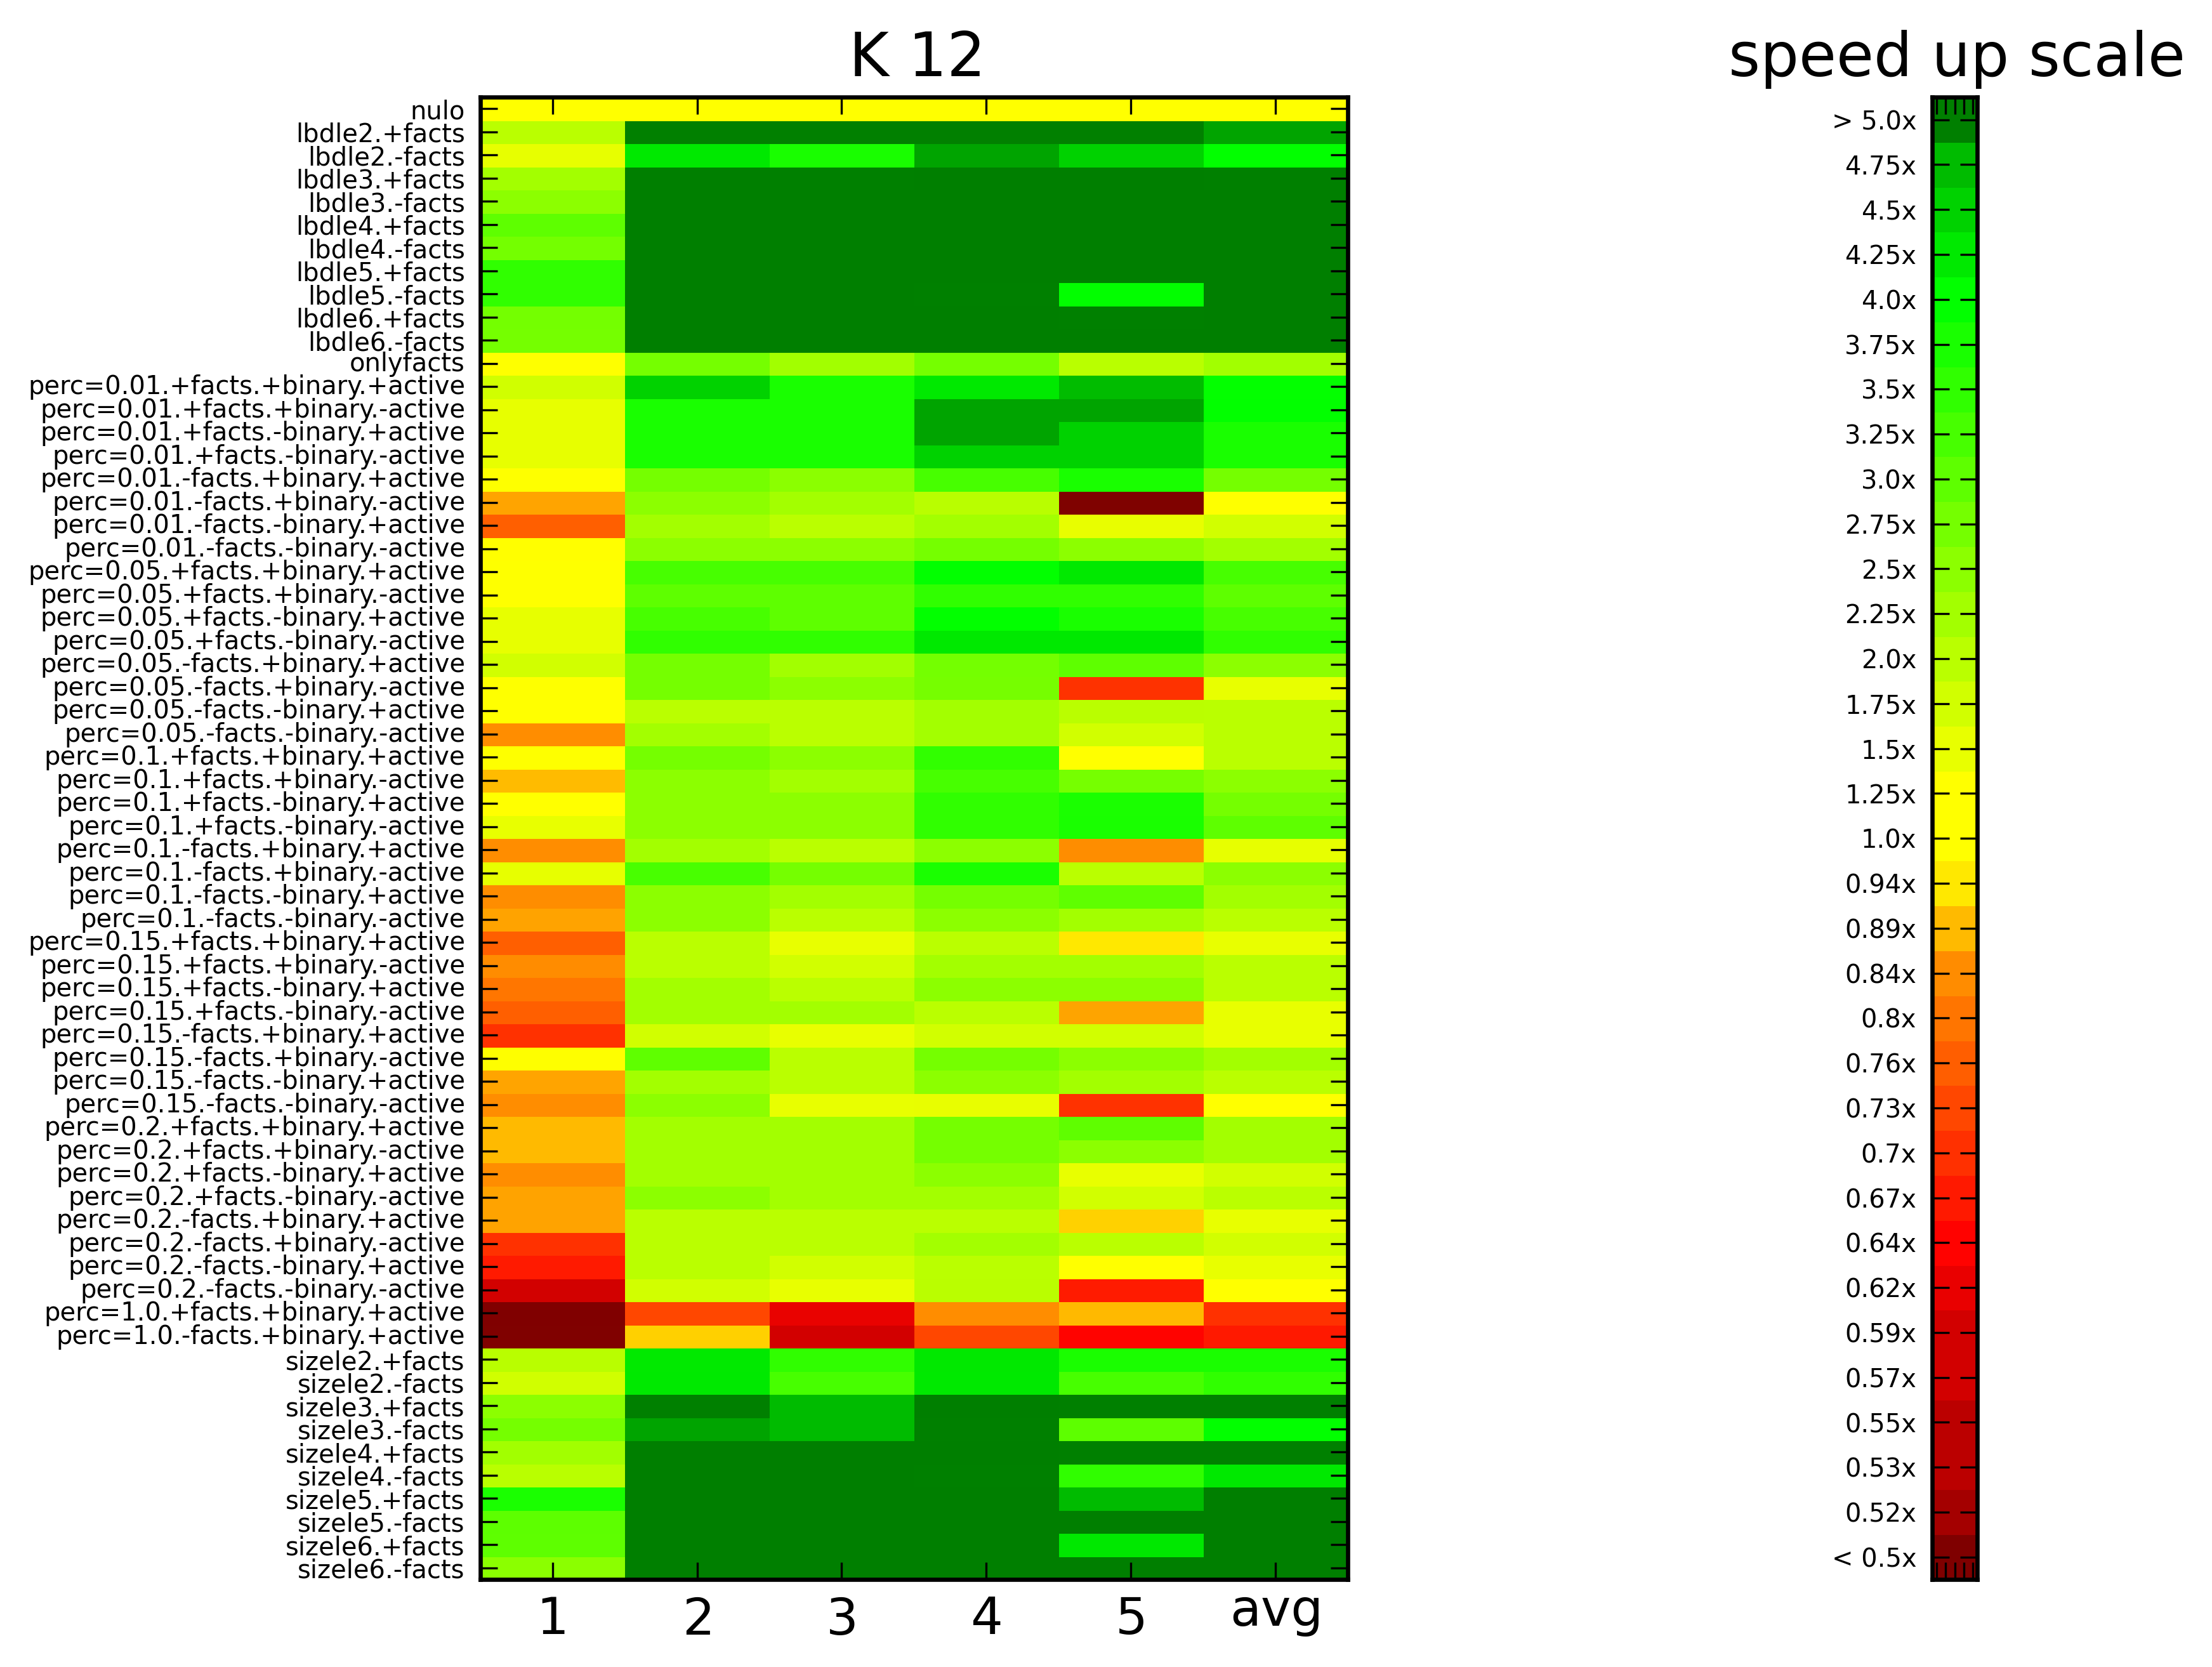
\includegraphics[scale=0.6]{resultados/k12_heat}
% 	%\caption{\emph{Workers}}
% \end{figure}
% \begin{figure}
% 	\centering
% 	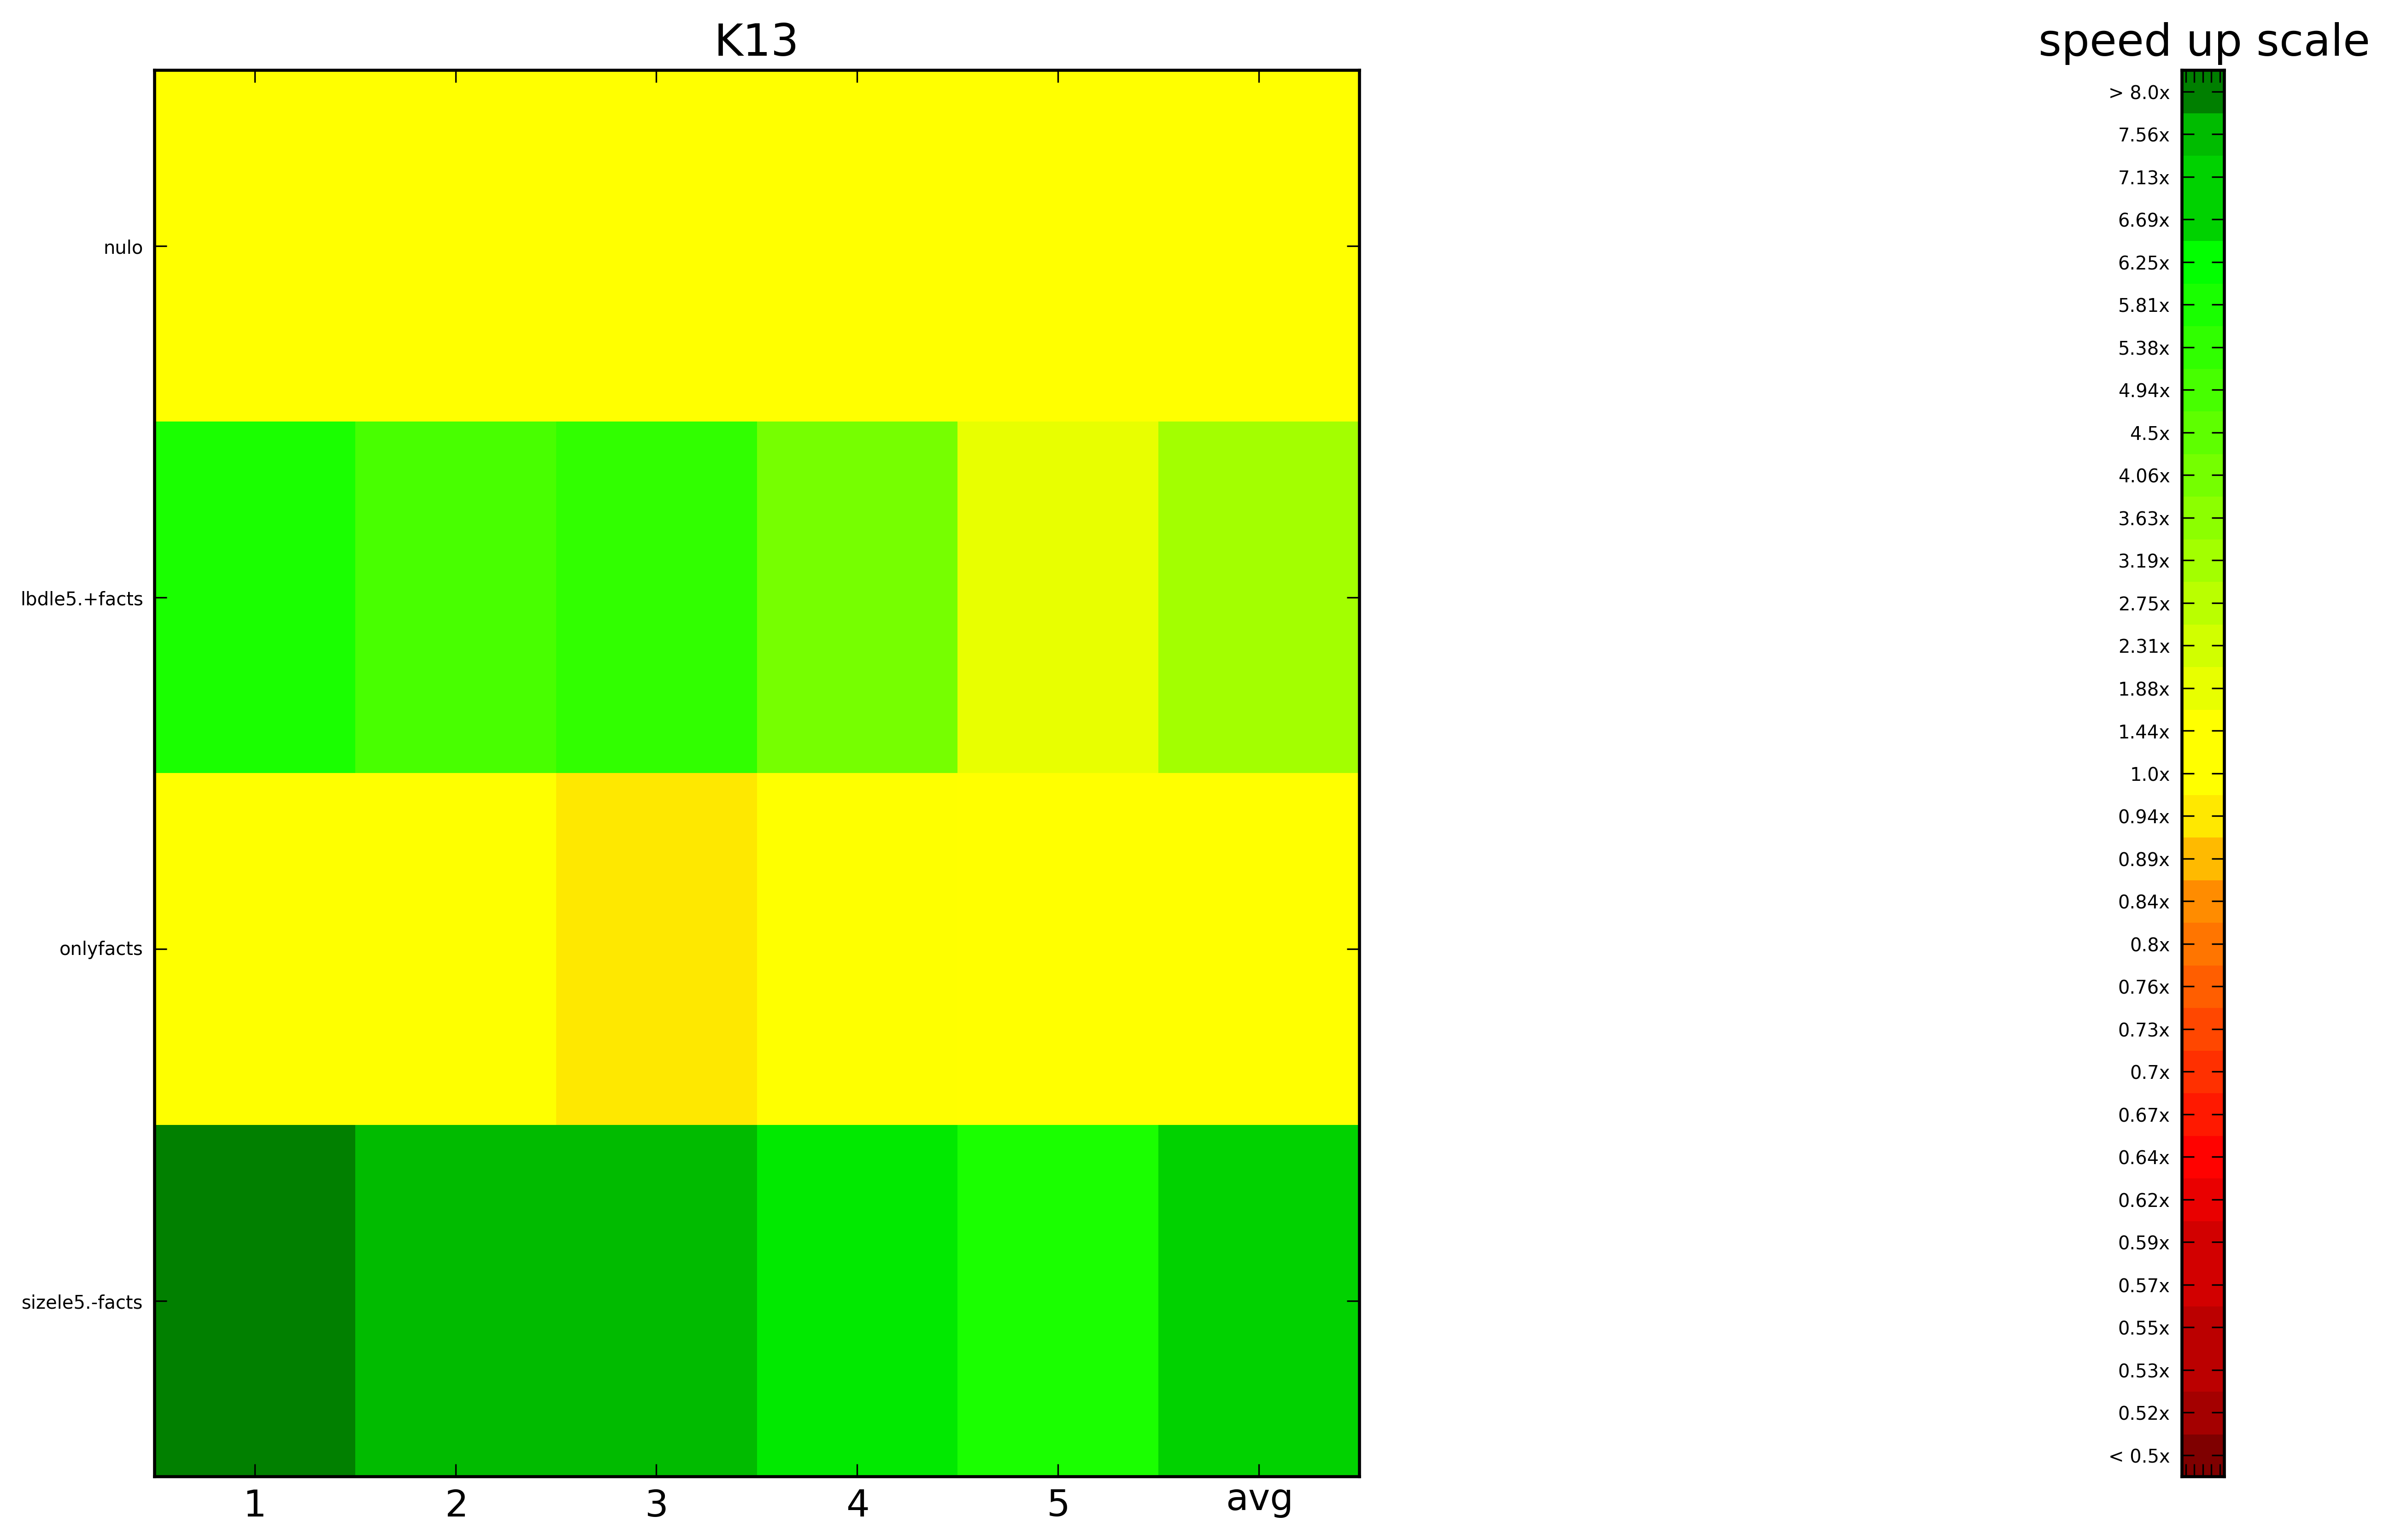
\includegraphics[scale=0.6]{resultados/k13_heat}
% 	%\caption{\emph{Workers}}
% \end{figure}

\hspace{-5em}
\begin{minipage}{\textwidth}
	\small
	\begin{tabular}{lrrr}
		\toprule
		criteria	&	worst speedup (x)	&	best speedup (x)	&	avg speedup (x) \\
		\cmidrule(r){1-4}
		lbdle2.+facts	&	0.68	&	4.91	&	1.97 \\
		lbdle2.-facts	&	0.71	&	3.84	&	1.24 \\
		lbdle3.+facts	&	0.78	&	5.16	&	1.41 \\
		lbdle3.-facts	&	0.75	&	5.71	&	1.69 \\
		lbdle4.+facts	&	0.64	&	6.80	&	1.68 \\
		lbdle4.-facts	&	0.79	&	5.83	&	1.83 \\
		lbdle5.+facts	&	0.69	&	6.74	&	1.64 \\
		lbdle5.-facts	&	0.77	&	5.25	&	2.14 \\
		lbdle6.+facts	&	0.76	&	5.79	&	1.95 \\
		lbdle6.-facts	&	0.70	&	6.08	&	1.94 \\
		\cmidrule(r){1-4}
		onlyfacts	&	\cellcolor{green}0.84	&	3.23	&	1.45 \\
		\cmidrule(r){1-4}
		perc=0.01.+facts.+binary.+active	&	\cellcolor{red}0.55	&	3.83	&	2.12 \\
		perc=0.01.+facts.+binary.-active	&	0.77	&	3.78	&	1.92 \\
		perc=0.01.+facts.-binary.+active	&	0.64	&	3.64	&	\cellcolor{red}1.19 \\
		perc=0.01.+facts.-binary.-active	&	0.65	&	3.50	&	1.39 \\
		perc=0.01.-facts.+binary.+active	&	0.74	&	2.73	&	1.91 \\
		perc=0.01.-facts.+binary.-active	&	0.69	&	2.38	&	1.30 \\
		perc=0.01.-facts.-binary.+active	&	0.74	&	\cellcolor{red}1.68	&	1.22 \\
		perc=0.01.-facts.-binary.-active	&	0.71	&	2.22	&	1.22 \\
		\cmidrule(r){1-4}
		sizele2.+facts	&	0.75	&	3.50	&	1.57 \\
		sizele2.-facts	&	0.81	&	3.32	&	\cellcolor{red}1.19 \\
		sizele3.+facts	&	\cellcolor{red}0.55	&	5.40	&	1.63 \\
		sizele3.-facts	&	0.75	&	3.87	&	1.39 \\
		sizele4.+facts	&	0.74	&	6.24	&	1.91 \\
		sizele4.-facts	&	0.72	&	4.21	&	1.81 \\
		sizele5.+facts	&	0.64	&	6.14	&	1.92 \\
		sizele5.-facts	&	0.58	&	\cellcolor{green}7.18	&	1.90 \\
		sizele6.+facts	&	0.72	&	5.08	&	2.17 \\
		sizele6.-facts	&	0.79	&	5.69	&	\cellcolor{green}2.61 \\
		\bottomrule
	\end{tabular}
	%\caption{Tiempo de ejecución (en segundos) distribuido vs. secuencial}
\end{minipage}



